\section{Data analysis}
As no data was surveyed by the authors, there will be no chapter on the experimental procedure. Instead, the focus will be on the analysis of the data, for most of which the framework ROOT was used. Data was provided from two sources:
\begin{enumerate}
	\item Monte Carlo simulations, separated by decay reaction.
	\item Actual data from the OPAL detector at the LEP collider.
\end{enumerate}


\subsection{Selection of cuts}
In a first step, the data from the Monte Carlo simulations is plotted over adequate range in the following parameters:
\begin{itemize}
	\item{\makebox[3cm][l]{\textbf{NCHARGED:}}The number of tracks visible in the drift chamber}
	\item{\makebox[3cm][l]{\textbf{PCHARGED:}}Energy of particles that left a track in the drift chamber}
	\item{\makebox[3cm][l]{\textbf{E\_ECAL:}}Energy deposited in the electromagnetic calorimeter}
	\item{\makebox[3cm][l]{\textbf{E\_HCAL:}}Energy deposited in the hadronic calorimeter}
	\item{\makebox[3cm][l]{\textbf{COS\_THET:}}Angle $\theta$ between created the positive lepton and the \\\makebox[3cm][l]{}incident positron beam}
	\item{\makebox[3cm][l]{\textbf{COS\_THRU:}}Angle between the thrust axis for hadronic events and the \\\makebox[3cm][l]{}incident positron beam}
\end{itemize}
These plots include the simulation events from decays to electrons, myons, tauons as well as quarks in similar amounts. These ratios are not a representation of the actual ratios as they would be expected in the real data, as the decay width of quarks is much greater than that of the three types of leptons. \\
To further improve comparability of the different data sets, all histograms were normed to an integral of 1. The resulting plots are shown in graphics !!ADD GRAPHS REF!!. Using these graphs, as well as the knowledge of the type of event, cuts are established which will later be used to separate the actual data, where there is no initial knowledge of the type of event.\\
Thus, for every type of educts, a cut is to be made with maximum possible efficiency in detecting the respective kind of event, as well as maximum purity, meaning that other events are falsely allotted as rarely as possible.

\newpage
\begin{figure}[h]
\centering
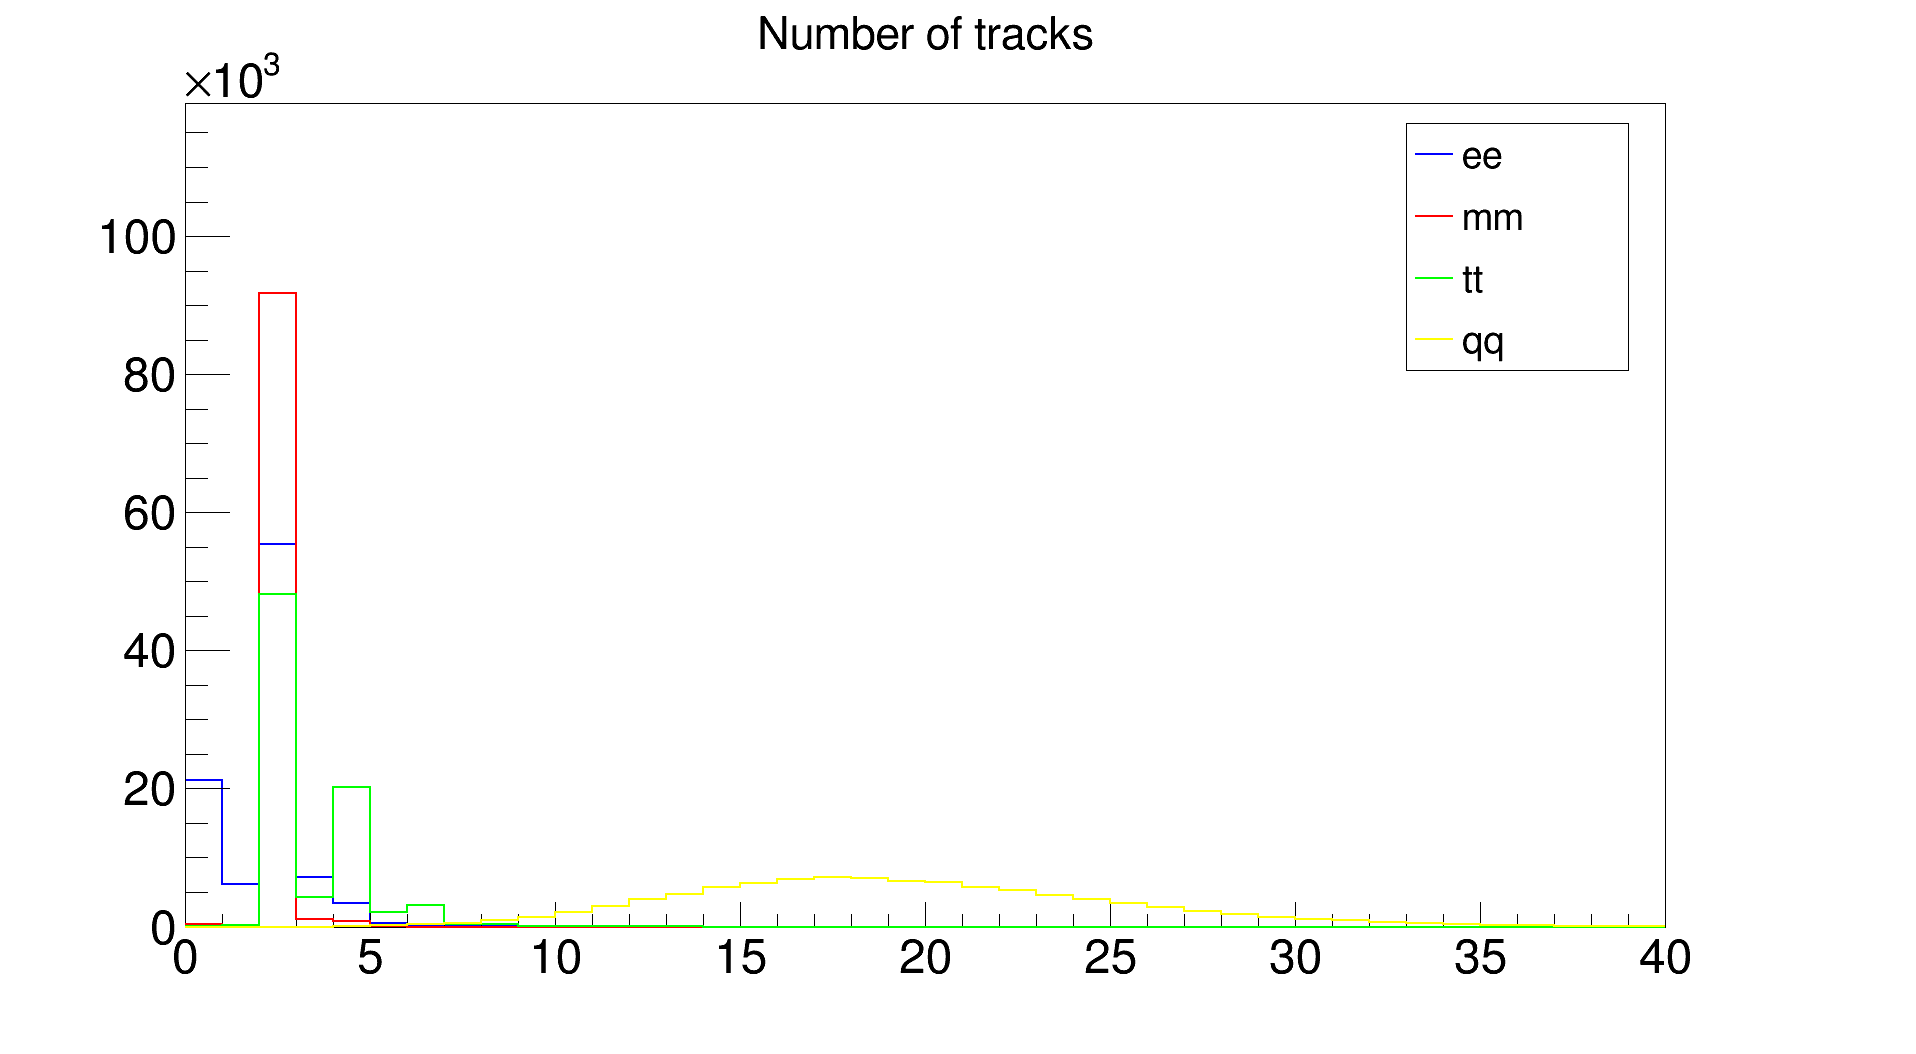
\includegraphics[width=1\linewidth]{../results/MC_results/nocut/Ncharged}
\caption[Ncharged in simulation data]{This figure shows the number of charged tracks in the simulation data. Almost all muon events leave two tracks. The peak is cut off to increase visibility of the other data.}
\label{fig:Ncharged}
\end{figure}

\subsubsection{Cuts in Ncharged}
Above figure suggests a good way to separate the data sets. In particular, all three lepton generations hardly ever leave more than 6 cuts, which then suggests the following cuts:

\begin{itemize}
	\item{\makebox[2.5cm][l]{\textbf{Lepton cuts:}} Ncharged $<7$}
	\item{\makebox[2.5cm][l]{\textbf{Quark cut:}} Ncharged $\ge8$}
\end{itemize}



\newpage
\begin{figure}[h]
\centering
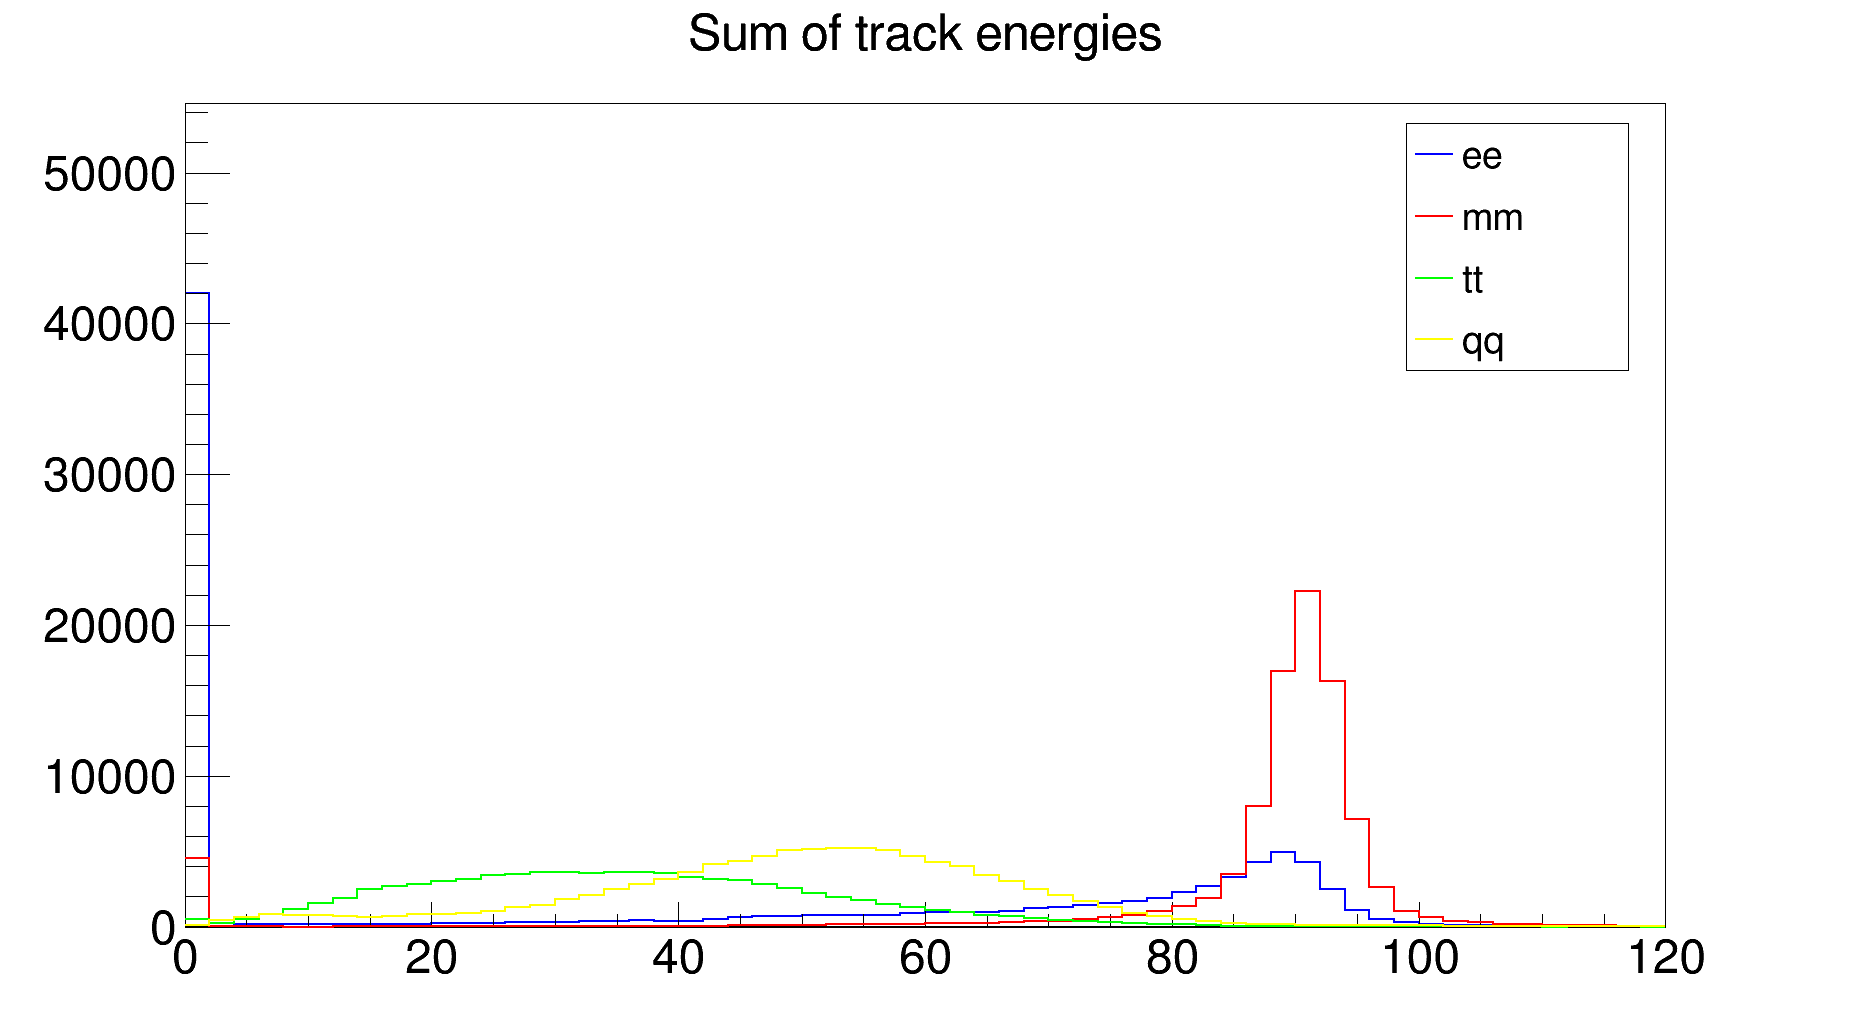
\includegraphics[width=1\linewidth]{../results/MC_results/nocut/Pcharged}
\caption[Pcharged in simulation data]{This figure shows the sum of track energies in the simulation data. }
\label{fig:Pcharged}
\end{figure}

\subsubsection{Cuts in Pcharged}
The separation of the data sets is less obvious in the Pcharged channel. Most datasets overlap, preventing the very clean cuts as they were in the Ncharged channel. However, since we have conveniently already cut against quarks in the Ncharged channel, we can ignore said dataset and separate tauons and muons as follows:
\begin{itemize}
	\item{\makebox[2.5cm][l]{\textbf{Muon cut:}} Pcharged $\le60$ GeV}
	\item{\makebox[2.5cm][l]{\textbf{Tauon cut}} Pcharged $>71$ GeV}
\end{itemize}

\newpage
\begin{figure}[h]
\centering
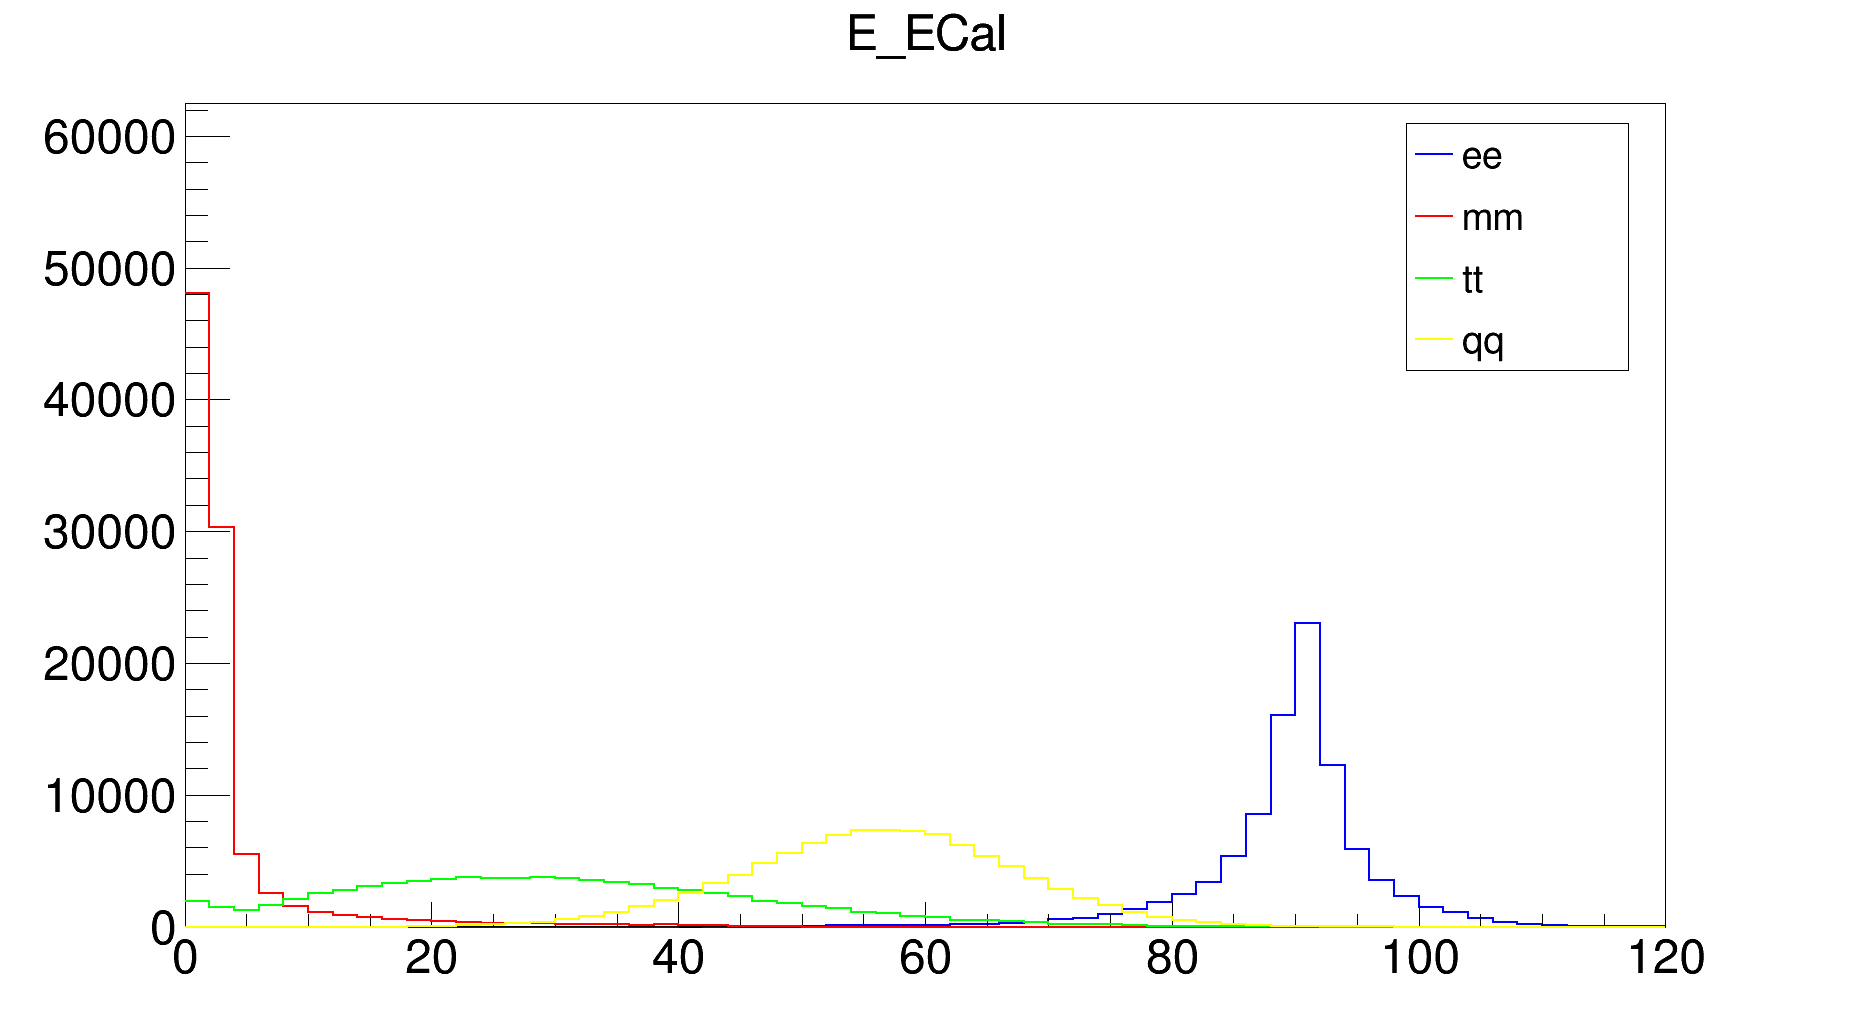
\includegraphics[width=1\linewidth]{../results/MC_results/nocut/E_Ecal}
\caption[E\_Ecal in simulations]{asd}
\label{fig:E_Ecal}
\end{figure}

\subsubsection{Cuts in E\_Ecal}
As has been the case for the cuts in Pcharged, we can ignore the quark data. Instead, cuts for all leptons are applied in order to separate the three kinds:

\begin{itemize}
	\item{\makebox[2.5cm][l]{\textbf{Electron cut}} E\_Ecal $\ge70$ GeV}
	\item{\makebox[2.5cm][l]{\textbf{Muon cut:}} E\_Ecal $<50$ GeV}
	\item{\makebox[2.5cm][l]{\textbf{Tauon cut:}} E\_Ecal $<60$ GeV}
\end{itemize}

\newpage
\begin{figure}[h]
\centering
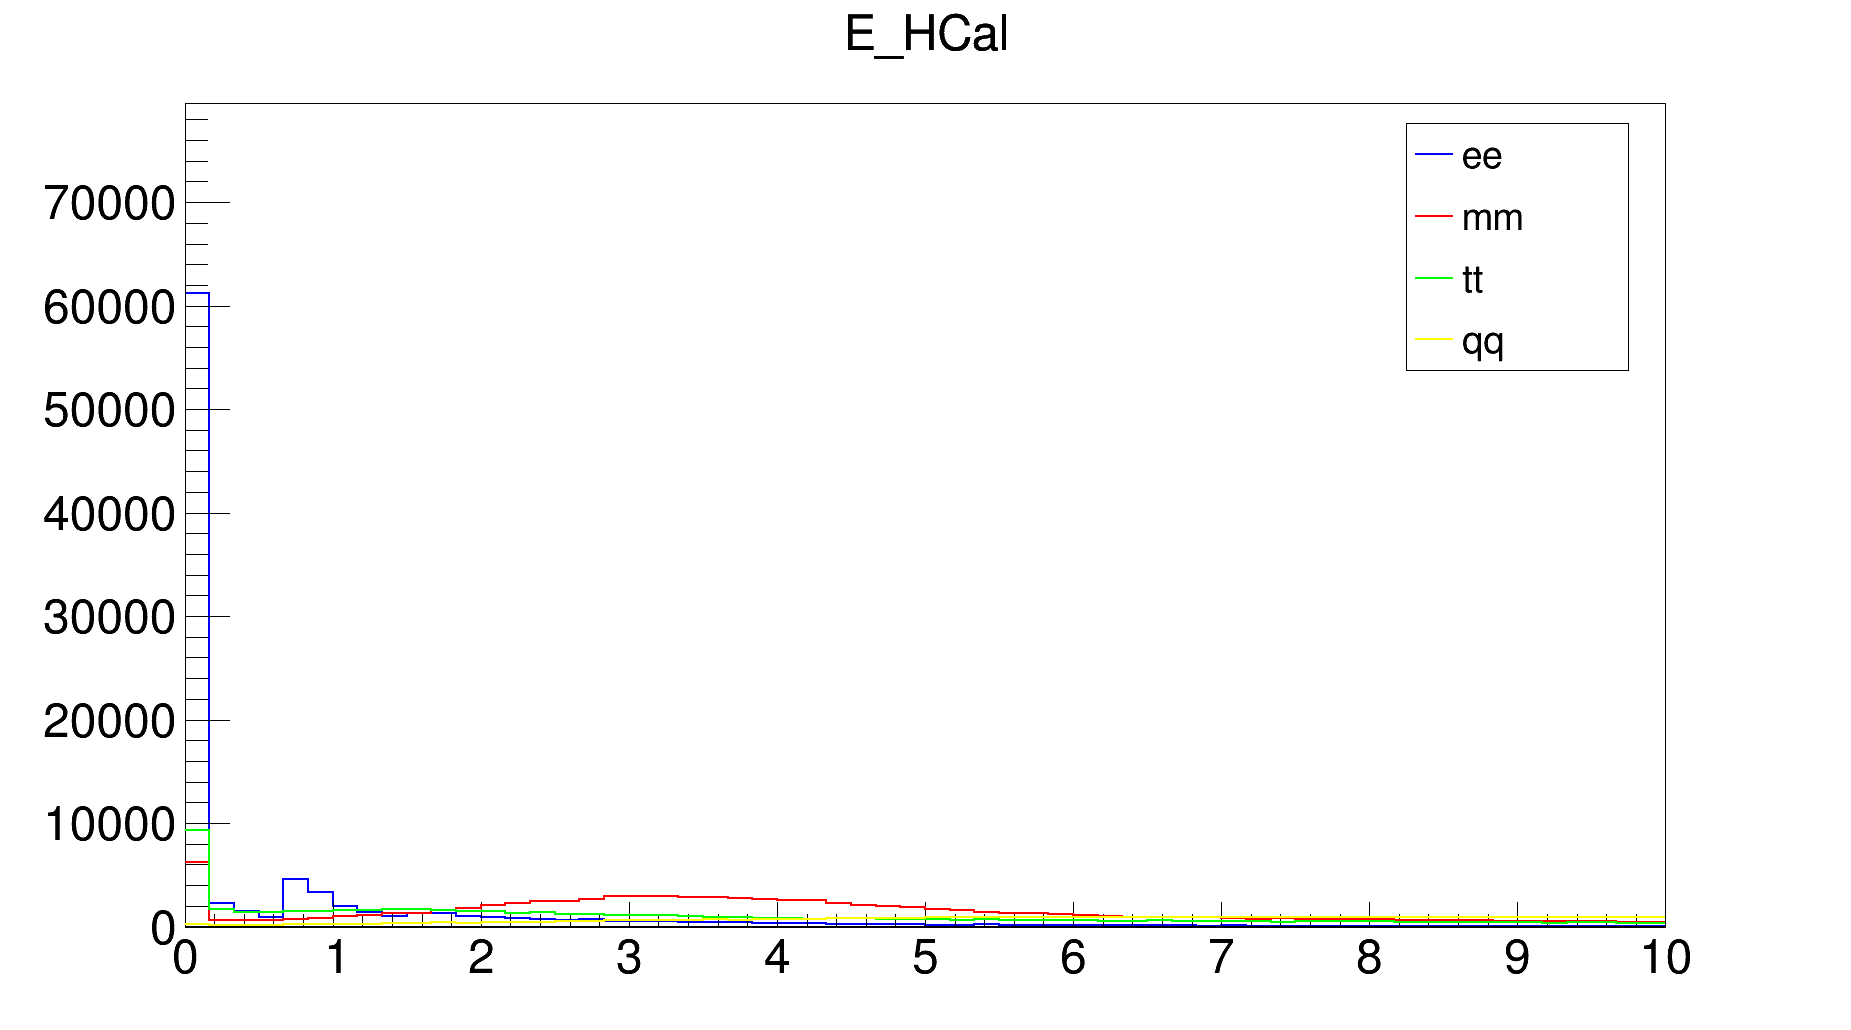
\includegraphics[width=1\linewidth]{../results/MC_results/nocut/E_Hcal}
\caption[E\_Hcal in simulation data]{a}
\label{fig:E_Hcal}
\end{figure}

\subsubsection{Cuts in E\_Hcal}
In the data from the hadronic calorimeter, the overlap between all four kinds of decay events is too great to allow for any kind of meaningful cuts.

\newpage
\begin{figure}[h]
\centering
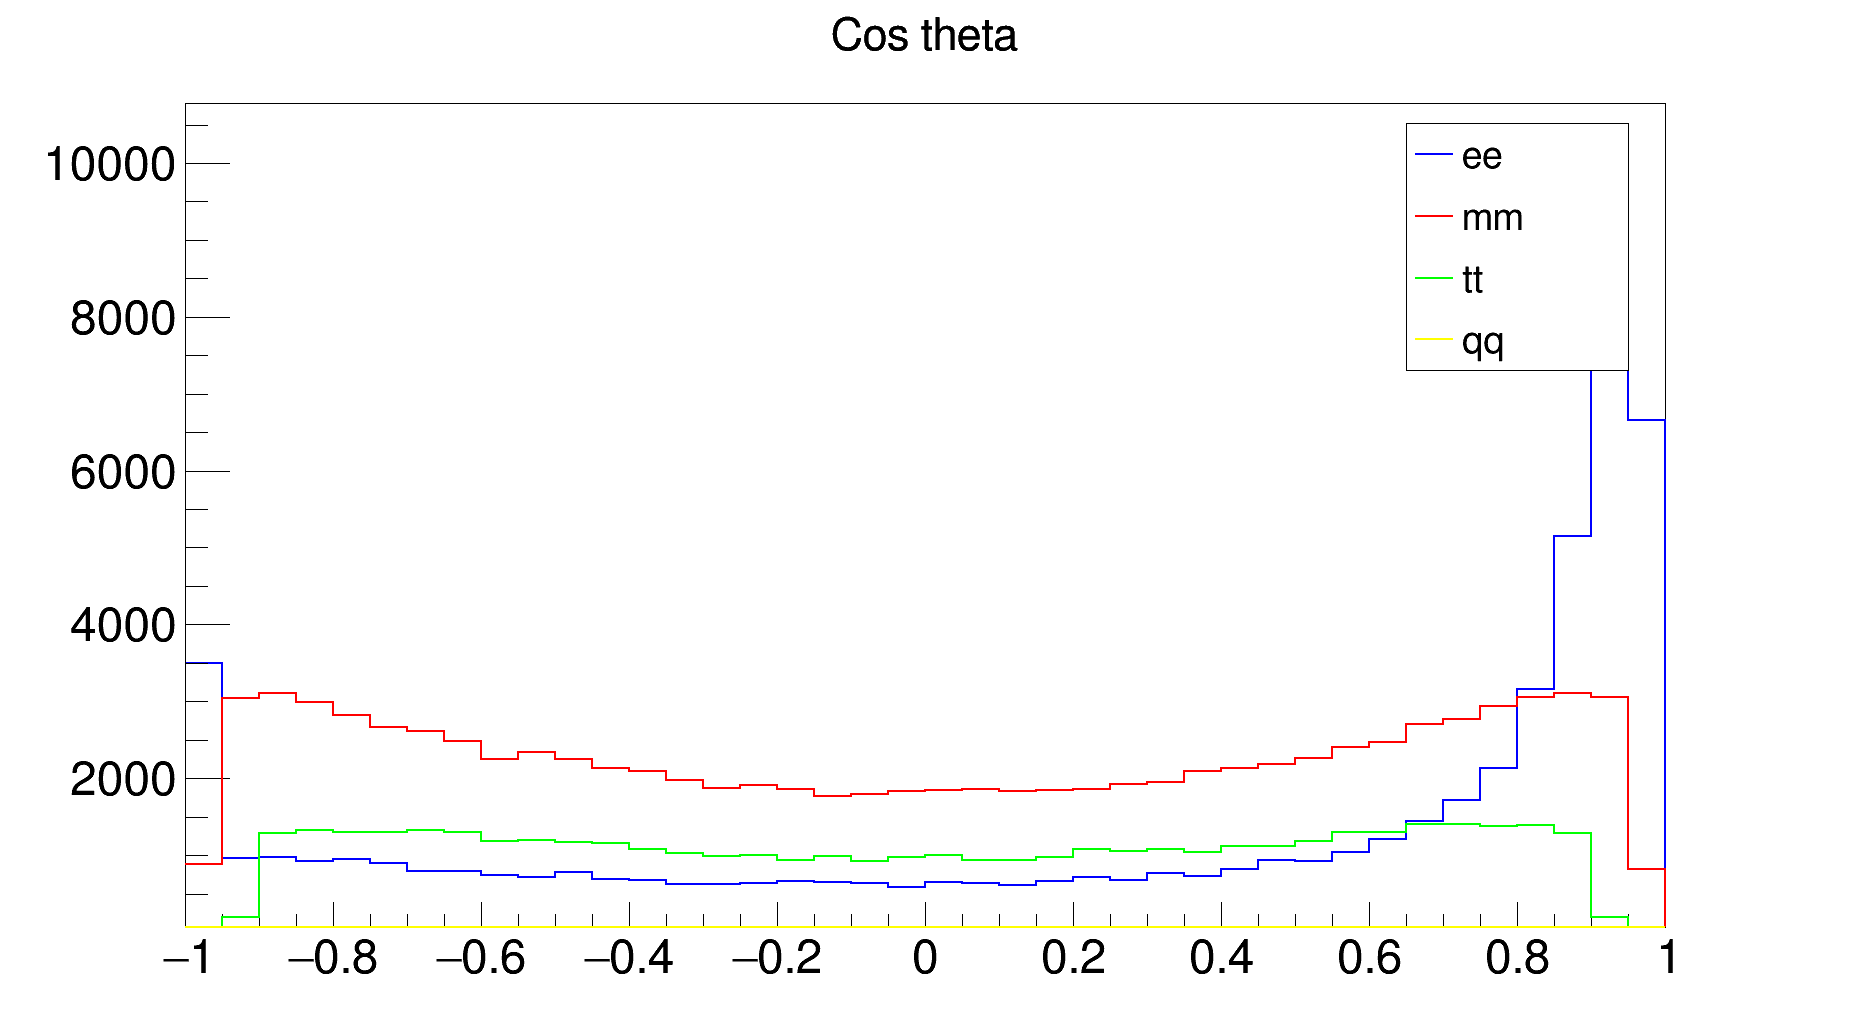
\includegraphics[width=1\linewidth]{../results/MC_results/nocut/cos_theta}
\caption[Cos\_theta in simulation data]{This figure shows the cosine of the angle between the beam and the direction of the created anti-lepton. Note the asymmetric peaks in the electron data, which will be discussed in the chapter on the separation of s- and t-channel.}
\label{fig:cos_theta}
\end{figure}

\subsubsection{Cuts in Cos\_theta}
As can be seen in figure \ref{fig:cos_theta}, the quark events are not assigned values of Cos\_theta within its natural boundaries from -1 to 1. This is due to the fact that they cause scattering jets, meaning that a well defined direction cannot be assigned. Leptonic events can also cause the creation of more than two particles. Furthermore, as there is no detection capacity in beam direction as well as for a very shallow angles, some regular events are also not assigned an angle. As a consequence, such events are listed with a Cos\_theta of $999.0$.\\
Since the electron data is later divided into s- and t-channel events, for which the Cos\_theta distribution is needed, it has to be ensured that the data is indeed valid. As there is no detection capacity for shallow angles to the beam direction, such events are cut off:

\begin{itemize}
	\item{\makebox[2.5cm][l]{\textbf{Electron cut}} $-0.9\le$ cos\_theta $\le0.9$}
\end{itemize}

\newpage
\begin{figure}[h]
\centering
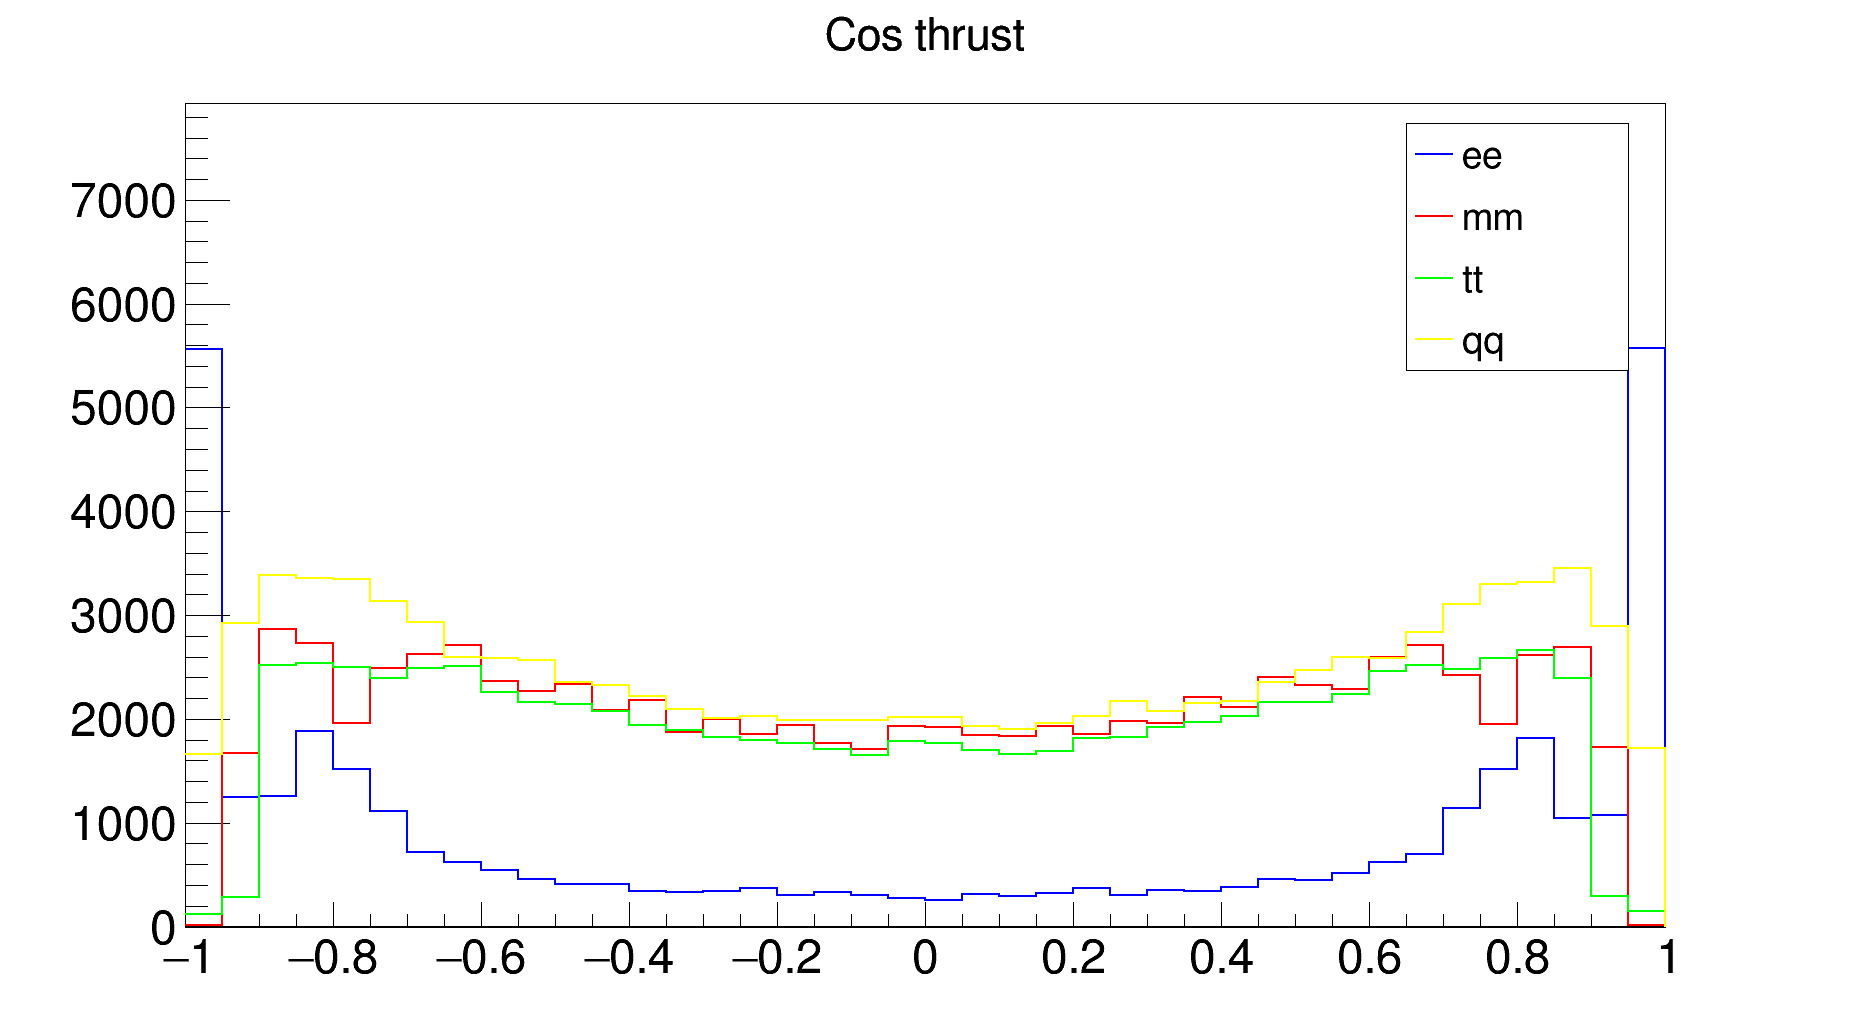
\includegraphics[width=1\linewidth]{../results/MC_results/nocut/cos_thru}
\caption[Cos\_thru in simulation data]{This figure shows the cosine of the angle between the beam and the thrust direction.}
\label{fig:cos_thru}
\end{figure}

\subsubsection{Cuts in Cos\_thrust}
Figure \ref{fig:cos_thru} suggests a cut to separate tauons from the rest of the particles, especially electrons, which often have have $cos_thrust>0.9$ or $cos_thrust<-0.9$

\begin{itemize}
	\item{\makebox[2.5cm][l]{\textbf{Tauon cut}} $-0.9\le$ cos\_thrust $\le0.9$}
\end{itemize}

The final cuts thus are
\begin{table}[H]\centering
	\begin{tabular}{@{}llllllll@{}}
		\toprule
		&			&Ncharged	&Pcharged [GeV]	&E\_Ecal [GeV] &Cos\_theta				&Cos\_thrust\\ 
		\midrule
		&Electron	&			&				&$\ge70$		&$\ge-0.9$ \& $\le0.9$	&\\
		&Muon		&			&$\le60$		&$<50$			&						&\\
		&Tauon		&$<7$		&$>71$			&$<60$			&						&\\
		&Quark		&$\ge8$		&				&				&						&$\ge-0.9$ \& $\le0.9$	\\
		\bottomrule
	\end{tabular}
	\caption[Table of cuts]{Cuts applied to separate the datasets. The Pcharged $!=0$ cut, which is discussed later, was applied to all datasets.}
\end{table}
\newpage
\subsection{Purity and the efficiency matrix}
These cuts are now applied to the simulated data, where the kind of event is known. This way, one can determine the efficiency and purity of the cuts and judge how well they work. 
The efficiency matrix is relatively easily calculated as
\begin{equation}
E_{ij}=\frac{n^{cut_{ij}}}{N_i}
\end{equation}
where the indexes $i$ and $j$ represent the kind of event. $n^{cut}_{ij}$ is thus the amount of events of type $i$ left over after applying the cut for type $j$ and $N_i$ is the overall number of events $i$ in the simulation data.
\begin{table}[H]\centering
	\begin{tabular}{@{}llllll@{}}
		\toprule
		&Events &$e^+e^-$&$\mu^+\mu^-$&$\tau^+\tau^-$&$q^+q^-$\\
		\midrule
		&Cut&&&&\\
		&$e^+e^-$&39.090&0.002&0.442&0.002\\
		&$\mu^+\mu^-$&0.018&90.171&0.611&0.001\\
		&$\tau^+\tau^-$&0.039&0.945&83.877&0.096\\
		&$q^+q^-$&0.007&0.001&0.687&98.970\\
		\bottomrule
	\end{tabular}
	\caption[Efficiency matrix]{Efficiency matrix of the applied cuts. All values are given in percent.}
	\label{tb:efficiency}
\end{table}

As these values describe event counts, they should be distributed binomially. According to Paterno \cite{binpaper}, the binomial error of such values is commonly calculated as
\begin{equation}
s_{E_{ij}}=\sqrt{\frac{E_{ij}\cdot(1-E_{ij})}{N_i}}
\end{equation}
where $N_i$ is the number of simulated events of the appropriate kind. This yields the following matrix

\begin{table}[H]\centering
	\begin{tabular}{@{}llllll@{}}
		\toprule
		&Events &$e^+e^-$&$\mu^+\mu^-$&$\tau^+\tau^-$&$q^+q^-$\\
		\midrule
		&Cut&&&&\\
		&$e^+e^-$&0.1593&0.0015&0.0236&0.0014\\
		&$\mu^+\mu^-$&0.0044&0.0969&0.0277&0.0010\\
		&$\tau^+\tau^-$&0.0065&0.0315&0.1307&0.0099\\
		&$q^+q^-$&0.0028&0.0011&0.0293&0.0322\\
		\bottomrule
	\end{tabular}
	\caption[Efficiency error matrix]{Errors of the efficiency matrix elements calculated under the assumption of binomial distribution. All values are given in percent.}
	\label{tb:efficiencyerr}
\end{table}

To calculate the purity, it has to be taken into account that the different events do not occur with the same probability in nature but are roughly equally represented in the simulated data. This is expressed by the branching ratio
\begin{equation}
BR_i=\frac{\Gamma_i}{\sum_{i,j}\Gamma_{i}}
\end{equation}
where $\Gamma_i$ is the partial decay width corresponding to event $i$. The partial decay widths of leptons $\Gamma_l=\unit{83.8}{\mega\electronvolt}$ and of quarks $\Gamma_q=\unit{1732}{\mega\electronvolt}$ are given in \cite{staatsex} without error.
Using this, the purity can be calculated as
\begin{equation}
P_i=\frac{BR_i\cdot E_{ii}}{\sum_{j}BR_j\cdot E_{ij}}
\end{equation}
which yields the following results:

\begin{table}[H]\centering
	\begin{tabular}{@{}lll@{}}
		\toprule
		&Cut&Purity\\
		\midrule
		&$e^+e^-$&0.9877\\
		&$\mu^+\mu^-$&0.9928\\
		&$\tau^+\tau^-$&0.9657\\
		&$q^+q^-$&0.9996\\
		\bottomrule
	\end{tabular}
	\caption[Purity of the cuts]{Purity of the cuts. All purities are above 95\%, indicating that the cuts work reasonably well.}
	\label{tb:purity}
\end{table}

\subsection{Calculation of the inverse efficiency matrix}
The efficiency matrix allows the calculation of the number of events after applying the cuts to a set of measurements where the kind of event is known:

\begin{equation}
\vec{N_c}=\boldsymbol{E}\cdot\vec{N}
\end{equation} 

where $\vec{N}$ is a vector whose components are the numbers of events of the four different kinds and $\vec{N_c}$ is a vector whose components are the number of events allocated to the four different cuts. 
In reality however, the kind of event is unknown and has to be determined by the cuts. Thus, the inverse of $\boldsymbol{E}$ can be used to calculate the number of actual events from the known number of events after the different cuts:
\begin{equation}
\vec{N}=\boldsymbol{E}^{-1}\cdot\vec{N_c}
\end{equation} 
The inverse of $\boldsymbol{E}$ is
\begin{table}[H]\centering
	\begin{tabular}{@{}llllll@{}}
		\toprule
		&Events &$e^+e^-$&$\mu^+\mu^-$&$\tau^+\tau^-$&$q^+q^-$\\
		\midrule
		&Cut&&&&\\
		&$e^+e^-$&0.1593&0.0015&0.0236&0.0014\\
		&$\mu^+\mu^-$&0.0044&0.0969&0.0277&0.0010\\
		&$\tau^+\tau^-$&0.0065&0.0315&0.1307&0.0099\\
		&$q^+q^-$&0.0028&0.0011&0.0293&0.0322\\
		\bottomrule
	\end{tabular}
	\caption[Inverse efficiency matrix]{The inverse of the efficiency matrix displayed in table \ref{tb:efficiency}.}
\end{table}
